\section{Qualitative Examples and Reproducibility}
\label{app:qualitative}

\subsection{Full trajectories}
Figure~\mainref{fig:qualitative} selects an unseen-I and a red-object episode where both baselines fail and \ours succeeds under GD. These illustrate changes in planning behavior; aggregate success is evaluated on the complete held-out sets. The source package supplies the first held-out target of test seed 2000 for each condition, and the displayed conditions are chosen by outcome. All methods share identical initial and goal observations. The panels use a consistent crop size to enlarge the movable objects, with every colored foreground element preserved.

Figures~\ref{fig:full_shape} and~\ref{fig:full_visual} provide additional CEM examples on the first held-out target of the same test seed: an unseen square and a red-agent shift. They show the complete trajectories and each method's prediction loss. These are separate from the GD examples in the main paper.

\begin{figure*}[!t]
 \centering
 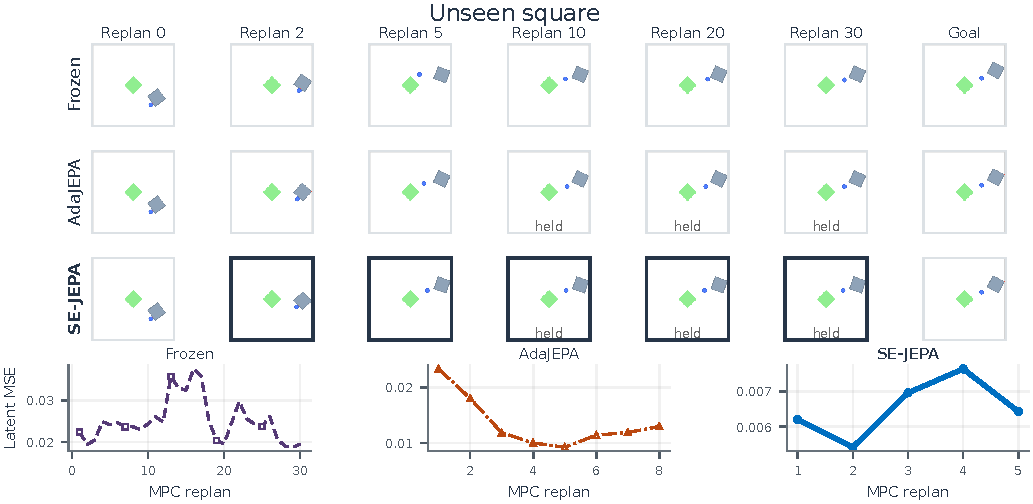
\includegraphics[width=\textwidth]{shape_full.pdf}
 \caption{Full unseen-square example with intermediate frames and prediction-loss traces. Frames marked held repeat the terminal state after success. \textbf{\ours} reaches the goal at replan five, AdaJEPA at replan eight, and the frozen model does not succeed within the budget.}
 \label{fig:full_shape}
\end{figure*}

\begin{figure*}[!t]
 \centering
 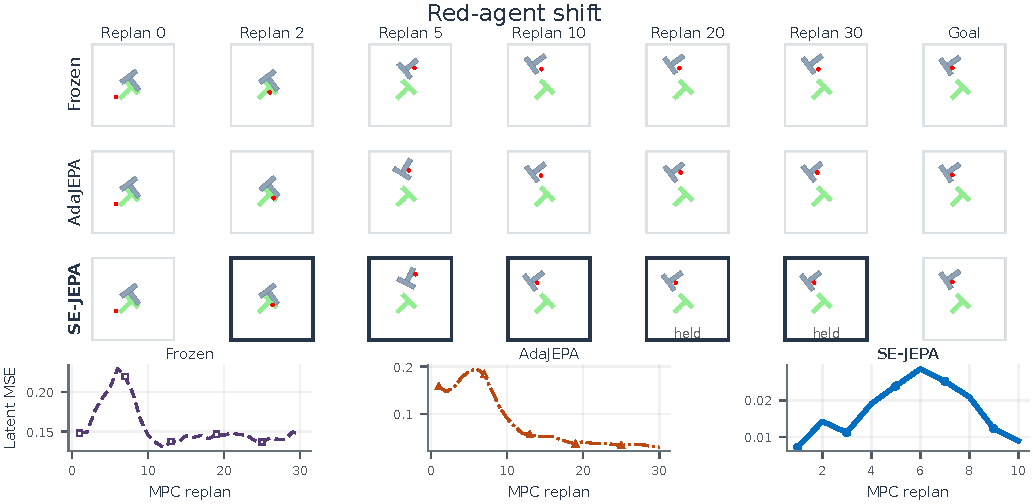
\includegraphics[width=\textwidth]{visual_full.pdf}
 \caption{Full red-agent example, replayed in the original simulator from the executed actions. \textbf{\ours} succeeds at replan ten; Frozen and AdaJEPA reach the 30-replan limit.}
 \label{fig:full_visual}
\end{figure*}

Each loss curve is measured in the latent space of its own model, so it describes how prediction error evolves within a method over the episode. Task success, judged in the shared simulator state, is the common yardstick across methods.

\subsection{Deformable rollout sequences}
Figures~\ref{fig:full_rope} and~\ref{fig:full_granular} expand the four deformable examples from Fig.~\mainref{fig:deform_qualitative}. Each row shows the start, every third push, and the goal over the same 15-push budget. The instances were selected from the repeated 50-instance learning stream where both baselines fail and the consolidated predictor succeeds. These third-pass examples illustrate slow-only planning; the aggregate results in Table~\mainref{tab:main} use the fourth pass. DINO-WM frames replay its recorded actions in the original FleX simulator. AdaJEPA and \ours frames were saved during planning, and the displayed CD values come from the original evaluation logs.

\begin{figure*}[p]
 \centering
 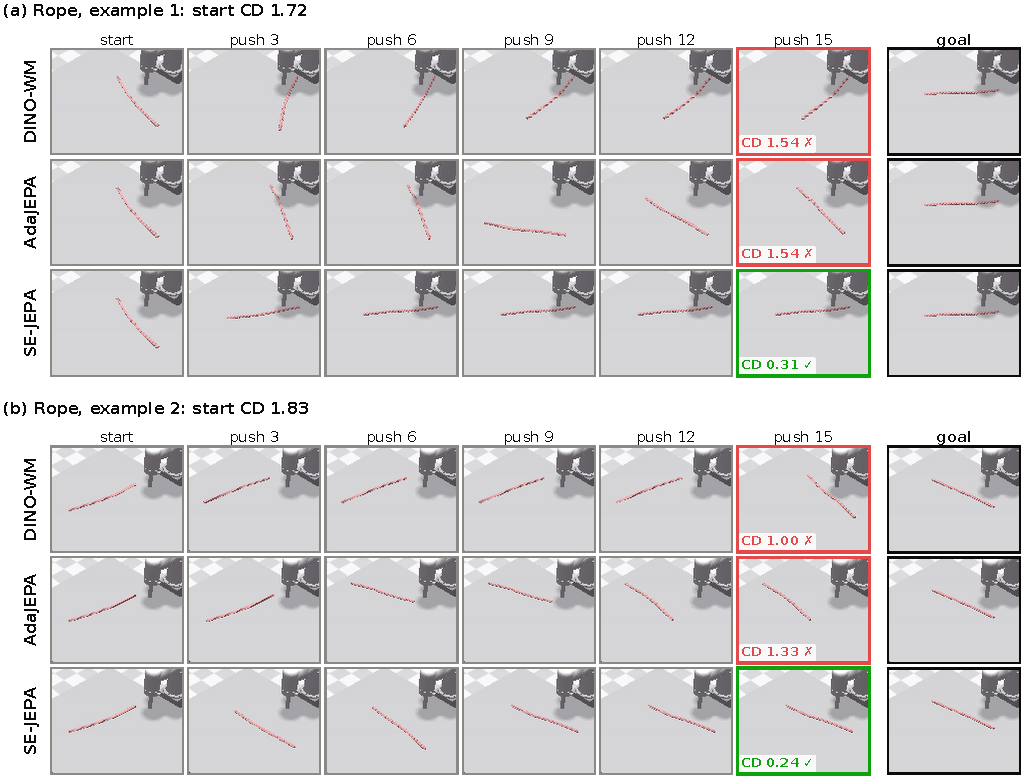
\includegraphics[width=\textwidth]{rope_full.pdf}
 \caption{\textbf{Complete rope manipulation sequences.} Two real instances, with DINO-WM, AdaJEPA and \ours sharing the initial state and goal. Columns show pushes 0, 3, 6, 9, 12 and 15, followed by the goal. Lower final Chamfer distance (CD) is better; the final-frame markers report task success. \ours uses the third-pass slow predictor without within-episode adaptation.}
 \label{fig:full_rope}
\end{figure*}

\begin{figure*}[p]
 \centering
 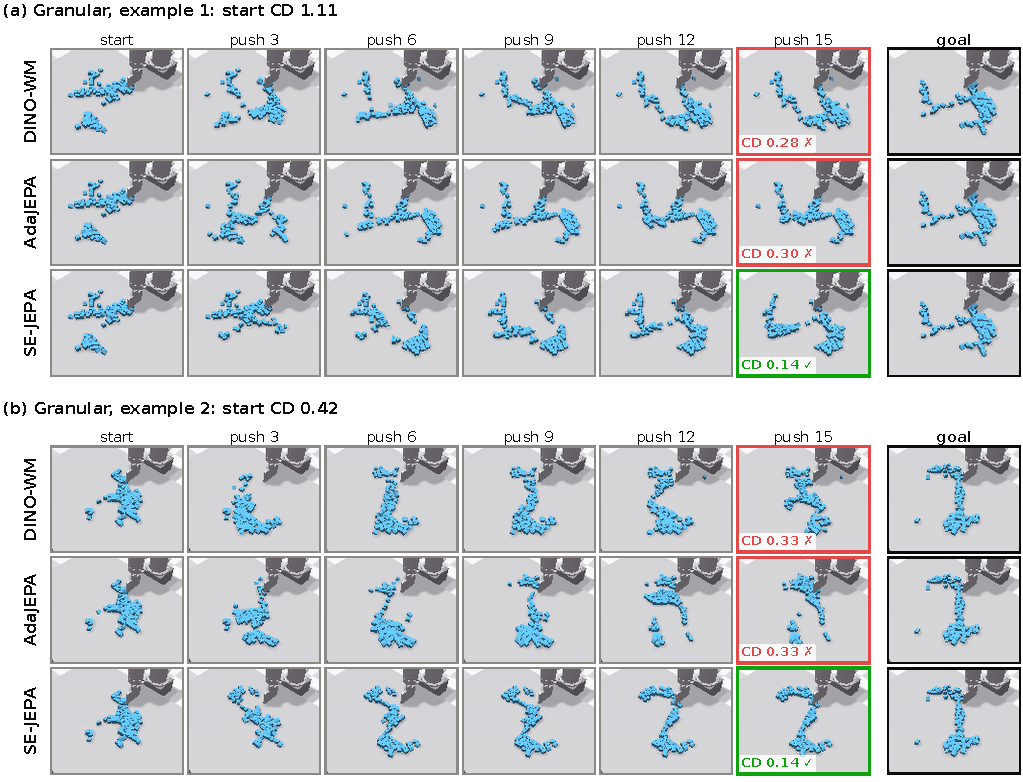
\includegraphics[width=\textwidth]{granular_full.pdf}
 \caption{\textbf{Complete granular manipulation sequences.} Two real instances under the same 15-push budget and reporting convention as Fig.~\ref{fig:full_rope}. All simulator frames are retained from the archived execution or action replay; the labels report recorded final CD and success. The third-pass slow predictor guides \ours.}
 \label{fig:full_granular}
\end{figure*}

\subsection{Reproducibility}
Tables and plots use the bundled reporting snapshot and the archived Drive experiment packages. The revised trajectory panels are rendered directly from the packages' simulator frames; the asset manifest records their source files and hashes. Success and Steps are computed from the final episode files and their run configurations. Offline world-model checkpoints record the upstream code revision, the epoch budget, the model configuration, and hashes of the adapter sources. Code, configurations, and learned memory states will be released.
